\newpage
\section{Theoretical Analysis}
\label{section:analysis}
Please present the theoretical analysis in this section. Moreover, please formally state the major theoretical results using theorem/proposition/corollary/lemma environments. Also, please clearly highlight your new proofs or extensions (if any).

\subsection{Proof for Benefits of Exploration with Demonstrations}

First, it is quite important to know whether adding the JS-divergence term as learning regularization could improve the agent policy eventually. So, starting from the surrogate function and the learning objective Eq. (3), one can prove the following Theorem:

\begin{figure}[ht]
    \center
    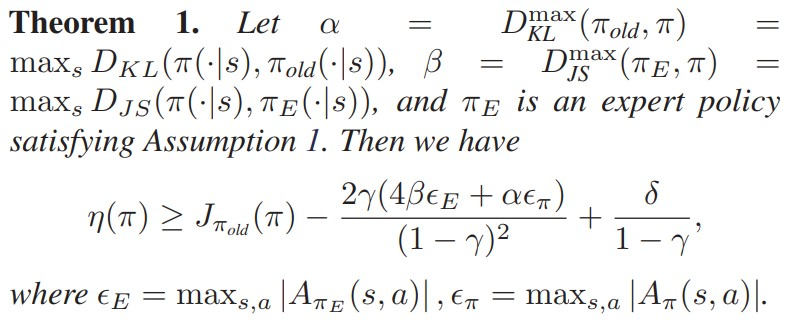
\includegraphics[width=8cm]
    {theorem1}
    \label{fig: theorem1}
\end{figure} 

Since it needs three pages to prove this inequality function of Theorem 1, and it has been provided by the paper’s supplement, so I decide to skip the details in this report. Most importantly, one can use Theorem 1 to further prove the benefits of adding the demonstration guided regularization term. \\
let $M_{i}(\pi)=J_{\pi_{i}}(\pi)-C_{\pi_{E}}D_{JS}^{max}(\pi,\pi_{E})-C_{\pi}D_{KL}^{max}(\pi,\pi_{i})+\hat{\delta}$ \\
where $C_{\pi_{E}}=\frac{8\gamma\epsilon_{E}}{(1-\gamma)^2}$, $C_{\pi}=\frac{2\gamma\epsilon_{\pi}}{(1-\gamma)^2}$, $\hat{\delta}=\frac{\delta}{1-\gamma}$. \\
And substitue the above $M_{i}(\pi)$ into the function of Theorem 1, we can derive:\\ $\eta(\pi_{i+1})\ge M_{i}(\pi_{i+1})$. \\
Then, since the KL divergence between the same policies will be zero, so \\ $\eta(\pi_{i})=M_{i}(\pi_{i})+C_{\pi_{E}}D_{JS}^{max}(\pi_{i},\pi_{E})-\hat{\delta}$. \\
Therefore, from these above two equations, one can derive: \\ $\eta(\pi_{i+1})-\eta(\pi_{i})\ge M_{i}(\pi_{i+1})-M_{i}(\pi_{i})-C_{\pi_{E}}D_{JS}^{max}(\pi_{i},\pi_{E})+\hat{\delta}$ \\
This result recalls the classic monotonic improvement guarantees for the policy gradient algorithm. But POfD brings another two terms $C_{\pi_{E}}D_{JS}^{max}(\pi_{i},\pi_{E})$ and $\hat{\delta}$. This implies when the agent follows the demonstrations, the JS divergence is close to zero, and therefore the advantage  term $\hat{\delta}$ from the reasonable assumption 1 can guarantee the monotonic policy improvement.


\subsection{Main Optimization Objective}

Since the JS divergence is quite hard to optimize, so this paper changes the way to optimize its lower bound which is given as Theorem 2:

\begin{figure}[ht]
    \center
    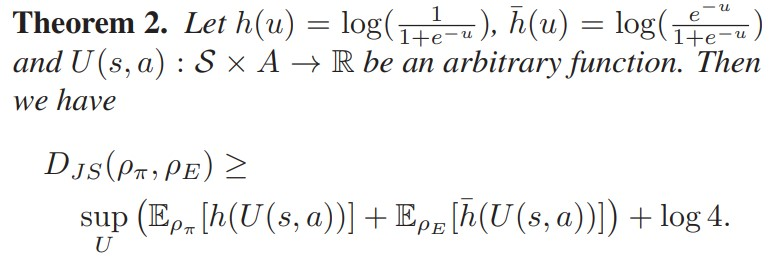
\includegraphics[width=8cm]
    {theorem2}
    \label{fig: theorem2}
\end{figure} 

Also, this theorem has been proved in the supplement provided by the paper author. Therefore, the occupancy measure matching objective can be written as

\begin{figure}[ht]
    \center
    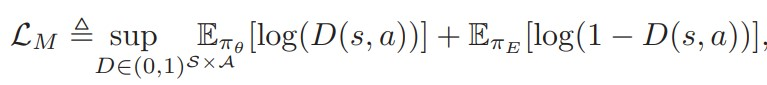
\includegraphics[width=8cm]
    {theorem2-1}
    \label{fig: theorem2-1}
\end{figure} 

That is, the supremum will range over $D(s,a)=\frac{1}{1+e^{-U(s,a)}}$ which is an arbitrary mapping function followed by a sigmoid activation funciton. And this objective can be regarded as the binary classification loss for distinguishing $\pi_{\theta}$ and $\pi_{E}$ w.r.t. state-action pairs sampled from the occupancy measure $\rho_{\theta}$ and $\rho_{E}$.  \\

To avoid the overfitting risks, this paper introduce the causal entropy $-H(\pi_{\theta})$ (\cite{ziebart2010modeling}). And thus the objective becomes the following form:

\begin{figure}[h!]
    \center
    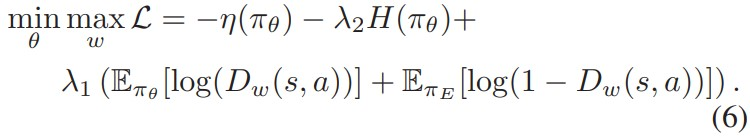
\includegraphics[width=8cm]
    {eq6}
    \label{fig: equation6}
\end{figure} 

It is actually a minimax problem similar to the GANs. In this POfD case, the true distribution is $\rho_{E}$, and the generator is to learn $\rho_{\theta}$. $D$ represents the discriminator parameterized by $w$, and we label the state-action pairs from expert as true ("1") while the policy as false ("0"). 

Moreover, by substituting Eq. (1) and Eq. (2) into Eq. (6), the objective becomes:

\begin{figure}[h!]
    \center
    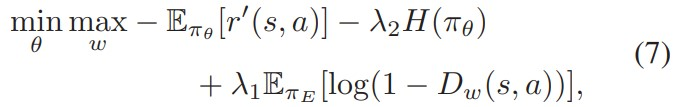
\includegraphics[width=8cm]
    {eq7}
    \label{fig: equation7}
\end{figure}

This function results in a dynamic reward reshaping mechanism. And the reshaped reward function is:   \\
$r^{\prime}(s,a)=r(s,a)-\lambda_{1}log(D_{w}(s,a))$ \\

It can augment the environment reward with aid of demonstrations. In other words, when the environment feedback is sparse, this reshaped reward can force the policy to generate similar trajectory as $\pi_{E}$. So, such way can make the agent to explore the environment more efficiently.

\subsection{POfD Algorithm}

The Eq. (7) can be optimized by alternately updating the parameters $w$ and $\theta$ of the discriminator and the agent policy, respectively. The overall optimization details are summarized in Alg. 1.
\begin{figure}[h!]
    \center
    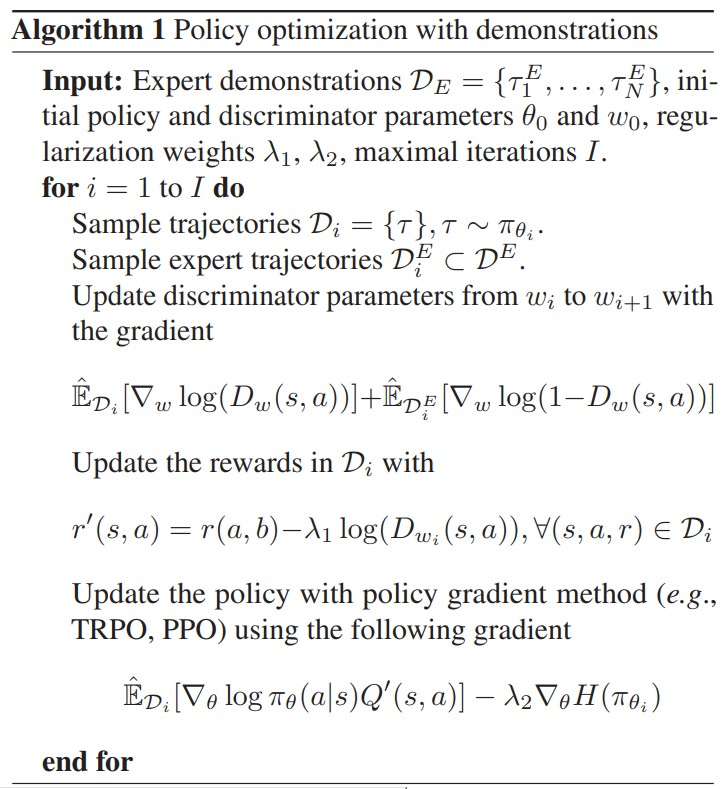
\includegraphics[width=7.5cm]
    {algorithm}
    \label{fig: algorithm}
\end{figure} 

Note that the reshaped policy gradient is given by:
\begin{figure}[h!]
    \center
    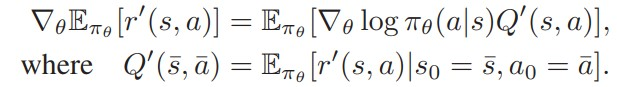
\includegraphics[width=8cm]
    {reshapeR}
    \label{fig: reshapeR}
\end{figure} 

And the gradient of causal entropy is:
\begin{figure}[h!]
    \center
    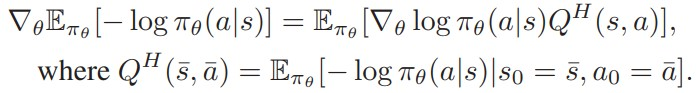
\includegraphics[width=8cm]
    {causalH}
    \label{fig: causalH}
\end{figure} 




